\section{Quantization}
\begin{example}
1-bit Gaussian: $X\sim\mathcal{N}(0,\sigma^2)$, 衡量指标: MSE=$\mathbb{E}\left[(X-\hat{X})^2\right]$. \\
Find $\hat{X}$ s.t. $\hat{X}$有两个取值, 使得MSE最小.
\end{example}
假设$\hat{X}\in\{a_1,a_2\}, \hat{X}=\begin{cases}
    a_1 & X\leq b \\
    a_2 & X>b
\end{cases}$ 则
$$MSE=\mathbb{E}[(X-\hat{X})^2]=\int_{-\infty}^bf(x)(x-a_1)^2dx+\int_b^{+\infty}f(x)(x-a_2)^2dx$$
可以解得$a_1=-\sqrt{\dfrac{2}{\pi}\sigma}, a_2=\sqrt{\dfrac{2}{\pi}\sigma}, b=\dfrac{a_1+a_2}{2}=0$. \\
i.e.
$$\hat{X}=\begin{cases}
    -\sqrt{\frac{2}{\pi}\sigma} & X\leq 0 \\
    \sqrt{\frac{2}{\pi}\sigma} & X>0
\end{cases}$$


\begin{example}
Quantization Region(1D): Aim: Given pdf $f_U(u)$ and alphabet size $M$, choose $\{R_j, 1\leq j\leq M\}$ and $\{a_j, 1\leq j\leq M\}$ to miminize MSE.
\begin{figure}[htbp]
    \centering
    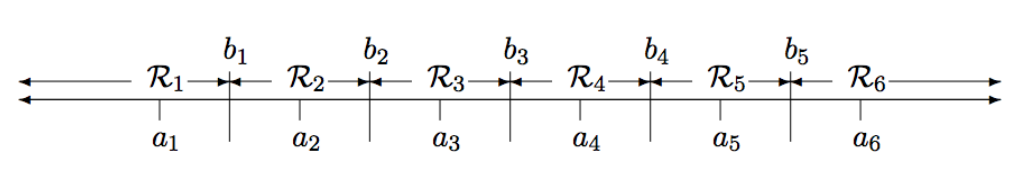
\includegraphics[width=\textwidth]{./figures/chapter8/1D_quantization.png}
\end{figure}
\end{example}
如图所示, 我们要选择 $a_i, b_i$, 分成两步解决: \\
1. Given $a_j$, choose $b_j$ such that $\mathbb{E}\left[(U-V)^2\right]$ is minimized.
\begin{align*}
\mathbb{E}\left[(U-V)^2\right] &= \sum_{j=1}^M \int_{\mathbf{R}_{\mathrm{J}}} f_U(u)\left(u-a_j\right)^2 d u \\
&= \sum_{j=1}^M \int_{b_{j-1}}^{b_j} f_U(u)\left(u-a_j\right)^2 d u \\
&= \cdots+\int_{b_{j-1}}^{b_j} f_U(u)\left(u-a_j\right)^2 d u+\int_{b_j}^{b_{j+1}} f_U(u)\left(u-a_{j+1}\right)^2 d u+\cdots
\end{align*}

Let $\dfrac{\partial \mathbb{E}\left[(U-V)^2\right]}{\partial b_j}=0$, we have $\left(\dfrac{\partial \int_{q(x)}^{g(x)} f(u) d u}{\partial x}=f(g(x)) \dfrac{\partial g(x)}{\partial x}-f(q(x)) \dfrac{\partial q(x)}{\partial x}\right)$

\begin{align*}
f_U\left(b_j\right)\left(b_j-a_j\right)^2 & -f_U\left(b_j\right)\left(b_j-a_{j+1}\right)^2=0 \\
2 b_j\left(a_{j+1}-a_j\right) & =a_{j+1}^2-a_j^2 \\
b_j & =\dfrac{a_j+a_{j+1}}{2}
\end{align*}

2. Choice of $\left\{a_j\right\}$ for given $\mathcal{R}_j$
\begin{align*}
\mathrm{MSE} &= \mathbb{E}\left[(U-V)^2\right]=\int_{-\infty}^{\infty} f(u)(u-v)^2 d u \\
&= \sum_{j=1}^M \int_{\mathcal{R}_j} f(u)\left(u-a_j\right)^2 d u \\
&= \sum_{j=1}^M \int_{\mathcal{R}_j} f(u)\left(u^2-2 a_j u+a_j^2\right) d u
\end{align*}

Let $\dfrac{\partial \mathbb{E}\left[(U-V)^2\right]}{\partial a_j}=0$, we have
\begin{align*}
& -2 \int_{\mathcal{R}_j} f(u) u d u+2 \int_{\mathcal{R}_j} f(u) a_j d u=0 \\
& \Longrightarrow a_j=\dfrac{\int_{R_j} u f(u) d u}{\int_{R_j} f(u) d u}
\end{align*}

总结步骤:
1. Choose $a_1<a_2<\cdots<a_M$ \\
2. set $b_j=\dfrac{a_j+a_{j+1}}{2}$ for $1 \leq j \leq M-1$ \\
3. Set $a_j=\dfrac{\int_{\mathcal{R}_j} u f(u) d u}{\int_{\mathcal{R}_j} f(u) d u}$, where $\mathcal{R}_j=\left(b_{j-1}, b_j\right]$ for $1 \leq j \leq M-1$ \\
4. Iterate on 2 and 3 until improvement is negligible.

It find local min, not necessarily global min.

\begin{example}
Quantization Region(2D): 和1D类似. \\
Given $\left\{\left(a_j, a_j^{\prime}\right)\right\}$, how to choose $\left\{\mathcal{R}_j\right\}$?
\begin{figure}[htbp]
    \centering
    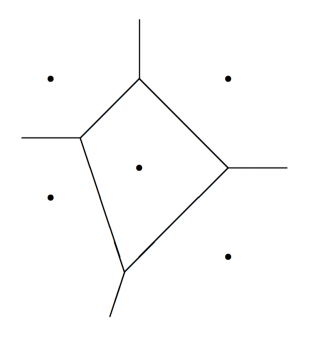
\includegraphics[width=0.3\textwidth]{./figures/chapter8/2D_quantization.png}
\end{figure}
\end{example}

Step1: 选择边界的划分方式: \\
1. The square error is $\left(u-a_j\right)^2+\left(u^{\prime}-a_j^{\prime}\right)^2$, the point $\left\{a_j, a_j^{\prime}\right\}$ which is the closest to $\left(u, u^{\prime}\right)$ in Euclidean distance should be chosen. \\
2. $\left\{\mathcal{R}_j\right\}$ contains points that are closer to $\left(a_j, a_j^{\prime}\right)$ than any other representation points, i.e., Voronoi regions. \\
Voronoi region 的划分: 在CG等领域已经有很多现成的算法, e.g.
\href{https://blog.csdn.net/yolon3000/article/details/78535183}{https://blog.csdn.net/yolon3000/article/details/78535183} \\
\href{https://zhuanlan.zhihu.com/p/459884570}{https://zhuanlan.zhihu.com/p/459884570}

Step2: 选择中心点的位置: \\
Given a set of Voronoi region, how to find the $\left\{a_j, a_j^{\prime}\right\}$? \\
Choose $\left\{a_j, a_j^{\prime}\right\}$ to be the conditional means within those regions.

和1D一样, 反复迭代直至收敛.
\begin{figure}[htbp]
    \centering
    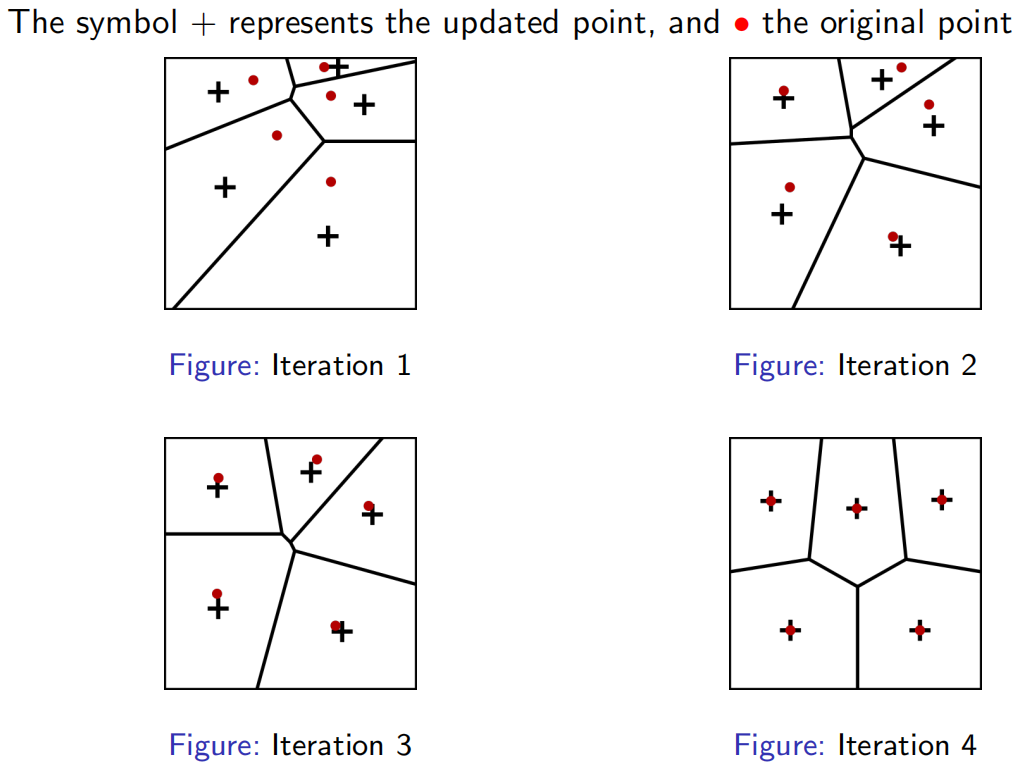
\includegraphics[width=\textwidth]{./figures/chapter8/2D_quantization_iter.png}
\end{figure}